\documentclass[11pt,titlepage]{article}
\usepackage{fullpage}
\usepackage{amsmath}
\usepackage{amssymb}
\usepackage{gensymb}
\usepackage[parfill]{parskip}
\usepackage{color}
\usepackage{bm}
\usepackage{graphicx}
\graphicspath{ {images/} }
\usepackage{tikz}
\usetikzlibrary{shapes,arrows,positioning,calc}
\usepackage{float}
\restylefloat{table}
\usepackage{array}
\tikzset{
    block/.style = {draw, fill=white, rectangle, minimum height=3em, minimum width=3em},
    sum/.style = {draw, fill=white, circle, node distance=1cm},
    input/.style = {draw=none},
    output/.style = {draw=none},
    coord/.style = {coordinate}
}

\author{Rane Brown \\ Kate Schneider}
\title{ECEN 4638: Lab W}
\date{\today}

\begin{document}
\maketitle
\tableofcontents
\listoffigures
\listoftables
\newpage

\section{Description}
The goal of this lab is to investigate the response of a two disc system when proportional control is used. System parameters are determined through experimental data collection and analysis, and the response of the physical system is compared to the expected response based on an LTI model.

\section{Setup}
In this experiment, we set up the Torsion Disc System to use two discs. The bottom disc is configured with 4 weights mounted at 6cm from the center rod, and the top disc is configured in multiple configurations for manual system excitation and data collection:
\begin{enumerate}
	\item 2 weights mounted at 6cm
	\item 2 weights mounted at 9cm
	\item 4 weights mounted at 6cm
\end{enumerate}
The final configuration (3) was also used for frequency analysis with the motor control on.

\section{System model}
	\subsection{LTI model}	
	With a two disc system, our model becomes more complex, as we must now take into consideration the position and velocity of each disk. The additional dynamics introduce the quantities $k$, the spring constant, and $c_2$, the damping ratio of the second disc. The two disc system can be modeled as:
	\begin{align}
		J_1\ddot \theta_1+c_1\dot \theta_1+k(\theta_1-\theta_2)=bu \\
		J_2\ddot \theta_2+c_2\dot \theta_2+k(\theta_2-\theta_1)=0
	\end{align}
	 The difference in position of the discs, $\beta$ is also of interest, where $\beta = \theta_1-\theta_2$. If we make this substitution, as well as substituting in angular velocity $\omega$ for $\dot \theta$, our system becomes:
	 \begin{align}
	 	J_1\dot \omega_1+c_1\omega_1+k\beta=bu \\
		J_2\dot \omega_2+c_2\omega_2-k\beta=0
	 \end{align}
	 
	\subsection{Transfer functions}
	For this experiment, there are three transfer functions of interest: the transfer function from the motor voltage control $u\mapsto\omega_1$, $u\mapsto\omega_2$, $u\mapsto\beta$. These can be determined by solving the system in the Laplace domain, or by using a state-space model of the system
	\begin{equation}
		\begin{bmatrix}
			\dot \omega_1\\
			\dot \omega_2\\
			\dot \beta
		\end{bmatrix}=
	  	\begin{bmatrix}
	    		-\frac{c_1}{J_1} & 0 & -\frac{k}{J_1} \\
		    	0 & -\frac{c_2}{J_2} & -\frac{k}{J_2}\\
			1 & -1 & 0
	  	\end{bmatrix}
		\begin{bmatrix}
			\omega_1\\
			\omega_2\\
			\beta
		\end{bmatrix}+
		\begin{bmatrix}
			\frac{b}{J_1}\\
			0\\
			0
		\end{bmatrix}
	\end{equation}
	and solving for the transfer functions with 
	\begin{align}
		\hat{x}(s) = (sI-A)^{-1}=b\hat{u}(s).
	\end{align}
	 Using the latter method, we obtain the transfer functions of interest:\\
	 \begin{align}
	  	H_{\omega_{1}u}(s)= \frac{\frac{b}{J_1}(s^2+\frac{c_2}{J_2}s+\frac{k}{J_2})}{s^3+(\frac{c_1}{J_1}+\frac{c_2}{J_2})s^2+(\frac{c_1}{J_1}\frac{c_2}{J_2}+\frac{k}{J_2}+\frac{k}{J_2})s+(\frac{k}{J_1}\frac{c_2}{J_2}+\frac{k}{J_2}\frac{c_1}{J_1})} \\[1em]
	  	H_{\omega_{2}u}(s)= \frac{\frac{b}{J_1}\frac{k}{J_2}}{s^3+(\frac{c_1}{J_1}+\frac{c_2}{J_2})s^2+(\frac{c_1}{J_1}\frac{c_2}{J_2}+\frac{k}{J_2}+\frac{k}{J_2})s+(\frac{k}{J_1}\frac{c_2}{J_2}+\frac{k}{J_2}\frac{c_1}{J_1})}\\[1em]
	  	H_{\beta u}(s)=\frac{\frac{b}{J_1}(s+\frac{c_2}{J_2})}{s^3+(\frac{c_1}{J_1}+\frac{c_2}{J_2})s^2+(\frac{c_1}{J_1}\frac{c_2}{J_2}+\frac{k}{J_2}+\frac{k}{J_2})s+(\frac{k}{J_1}\frac{c_2}{J_2}+\frac{k}{J_2}\frac{c_1}{J_1})}
	  \end{align}\\
	  It should be noted that these transfer functions have the same poles and different zeros, as is expected. In this lab, we are interested in a collocated system in which sensing and actuation occur at the same place. For this reason, $\omega_1$ is fed back into our system, and the transfer function of greatest interest to us is $H_{\omega_{1}u}(s)$.

\section{Manual determination of system parameters}
	System parameters spring constant $k$ and damping ratio $c_2$ can be determined by manual oscillation of the system and Matlab analysis of the results. To determine these parameters, we manually oscillate the bottom disc and record the position of both the top and bottom disc. The position information of each disc is recorded in LabView, and is imported into Matlab for processing using the \texttt{accel\_fir.m} and \texttt{conv\_delay.m} scripts to obtain filtered position data. We can then use a least-squares approach to determine $c_2$ and $k$ for each configuration of weights that was tested. The least-squares evaluation is set up as:
	\begin{align}
	\begin{bmatrix}
		\dot \theta_2 & \theta_1-\theta_2
	\end{bmatrix} 
	\begin{bmatrix}
		c\\
		k
	\end{bmatrix}&=
	\begin{bmatrix}
		-J_2\ddot \theta_2
	\end{bmatrix}\\
	\bm{A}x&=\bm{B}
	\end{align}
	Where $c_2$ and $k$ can be found by $x=\bm{A}$\textbackslash$\bm{B}$. The results for the various weight configurations of disc 2 are:
	    \begin{table}[H]
            \centering
            \begin{tabular}{|m{5cm}|m{3cm}|m{3cm}|m{3cm}|} 
                \hline
                Weight distribution disc 2 & $J_2$ & $c_2$ & $k$ \\ 
                \hline
                2 weights at 6cm & 0.0058 & 0.0093 & 2.059\\
                \hline
                2 weights at 9cm & 0.0103 & 0.018 & 2.1231\\
                \hline
                4 weights at 6cm & 0.0097 & 0.0107 & 2.2306\\
                \hline
            \end{tabular}
            \caption{Data Collection Parameters} \label{table:data_param}
        \end{table}
         Taking the average, we obtain $c_2 = 0.0107$ and $k=2.1822$.
	
\section{System stability}
	\subsection{Root locus analysis}
	From the transfer functions for our system as well as the manually determined system parameters, we can estimate our system's stability before the introduction of a controller. This is accomplished by plotting the root locus of the system to determine whether, and at what gain, the system becomes unstable. The root locus plot for the transfer function $H_{\omega_{1}u}(s)$ with 2 weights at 6cm for the top disc is shown below. 
	\begin{figure}[H]
        \centering
        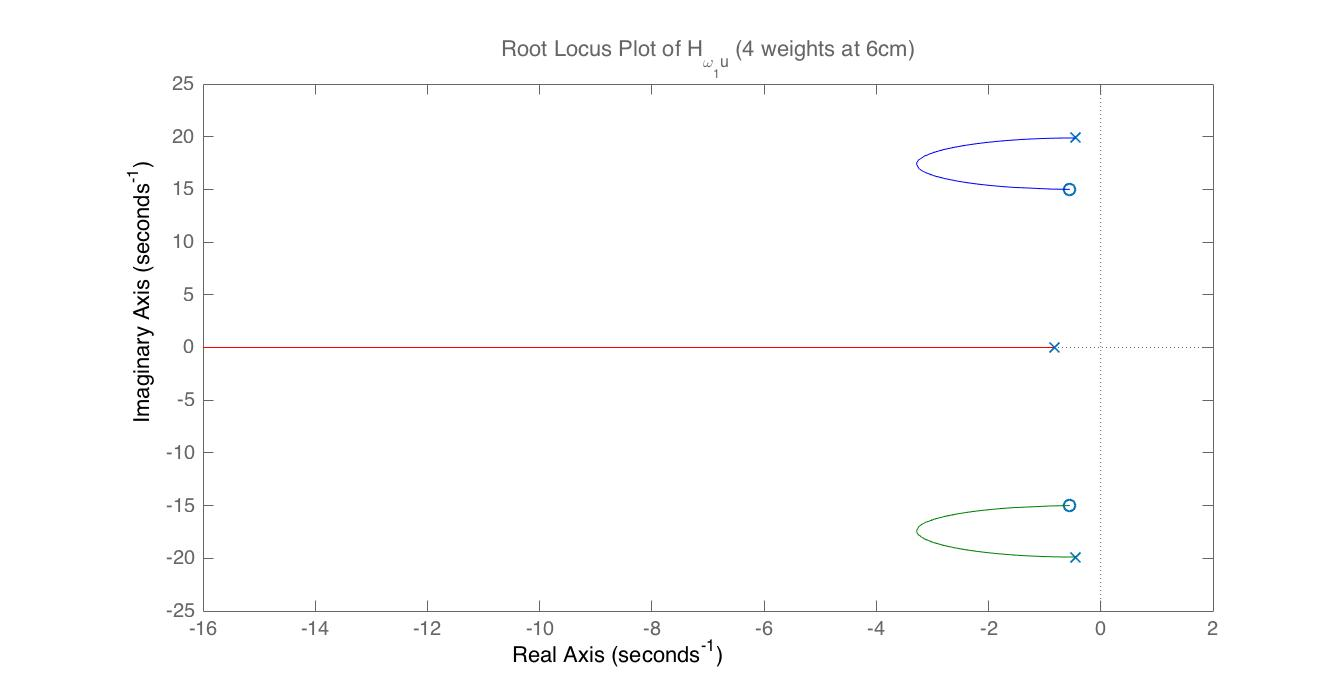
\includegraphics[trim={6cm 0 1cm 1cm},clip,origin=c,scale=0.26]{rlplot_4w_6cm_2disks}
        \caption{Root Locus Plot $H_{\omega_{1}u}$}
        \label{fig:disc_sys}
    \end{figure}
     From the root locus plot, it can be seen that the system, theoretically, should not go unstable no matter how large the gain is. However, we know from previous experiments that this is not the case. Our system has additional dynamics at play which are not accounted for in our model. The roots of our system occur at $s=-0.4456 \pm 19.9j$ and $s=-0.827$.\\

     We can also look at the root locus plots of the transfer functions $H_{\omega_{2}u}(s)$ and $H_{\beta u}(s)$, to see how the different zeros affect stability. These plots are included below.
       \begin{figure}[H]
            \centering
            \begin{minipage}{.5\textwidth}
                \centering
              	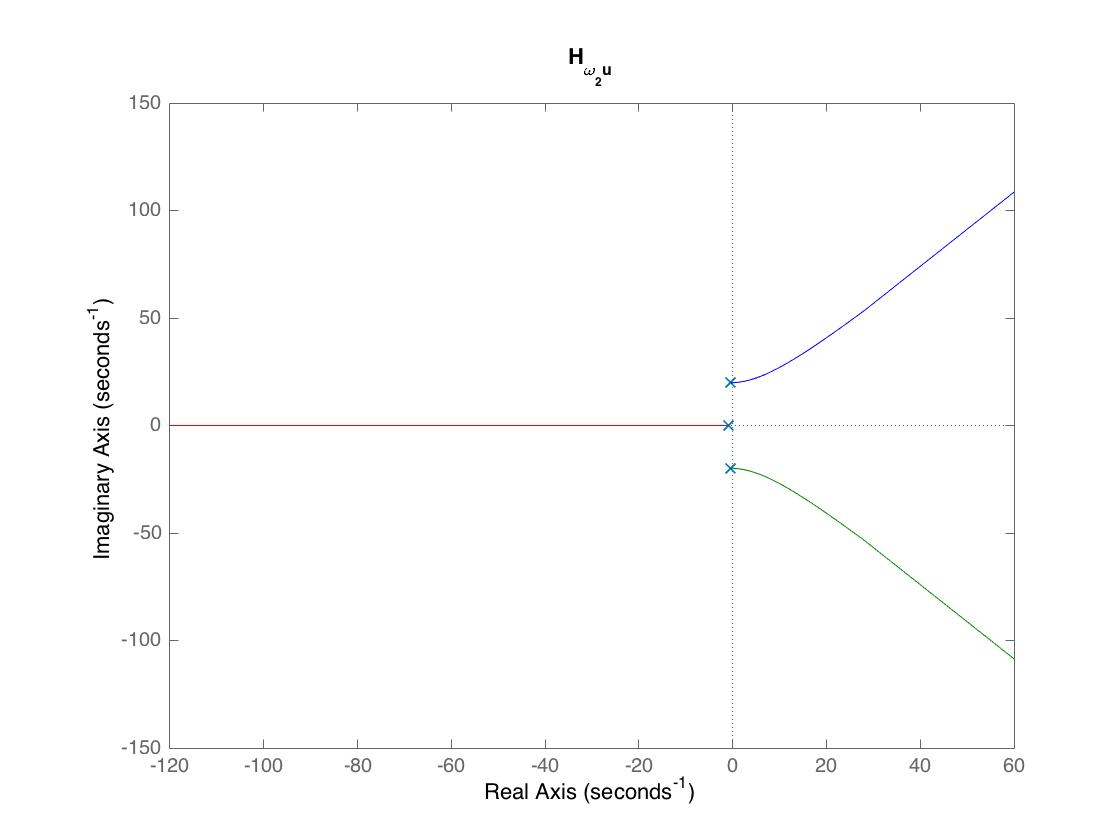
\includegraphics[trim={6cm 0 0 0},clip,origin=c,scale=0.25]{rlplot_w2}
            	\caption{Root Locus Plot $H_{\omega_{2}u}$}
           	\label{fig:disc_sys}
            \end{minipage}%
            \begin{minipage}{.5\textwidth}
                \centering
                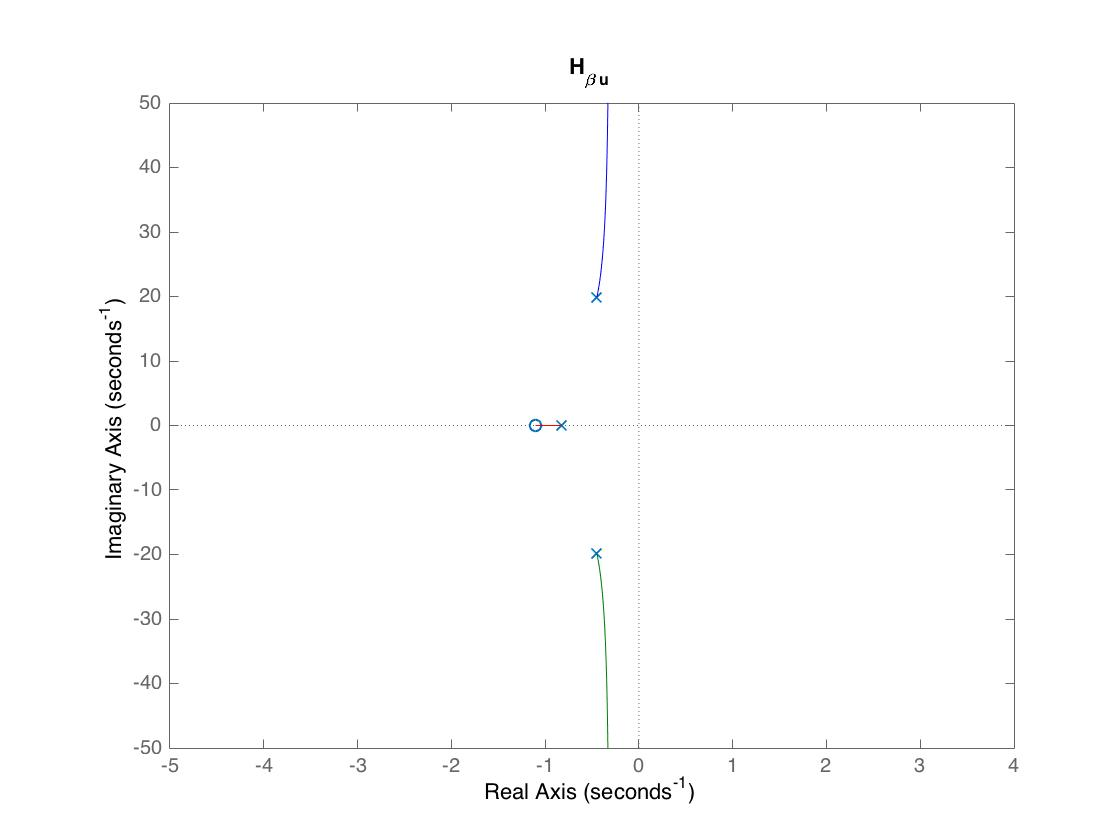
\includegraphics[trim={6cm 0 0 0},clip,origin=c,scale=0.25]{rlplot_B}
            \caption{Root Locus Plot $H_{\beta u}$}
            \label{fig:disc_sys}
            \end{minipage}%
       \end{figure}
       
	
	\subsection{Routh's stability criterion}
	Another way to determine system stability is via Routh's stability criterion. This can also be calculated for our system using our manually determined parameters $c_1$, $c_2$, and $k$:\\\\
	$\begin{matrix}
		s^3: & 1 & 396.182\\
		s^2: & 1.72 & 327.05\\
		s^1: & 206.0367 & 0\\
		s^0: & 327.05 & 0
	\end{matrix}$\\

	 Since there are no sign changes in the first column of our Routh array, we can confirm that the theoretical system should be stable.

	\subsection{Theoretical Bode analysis}
	With our system parameters, we can also plot the frequency response of the transfer functions of interest. These plots are included below for comparison to the frequency response determined experimentally, which is discussed further in section \ref{sec:bode}. 
	
	\begin{figure}[H]
            \centering
            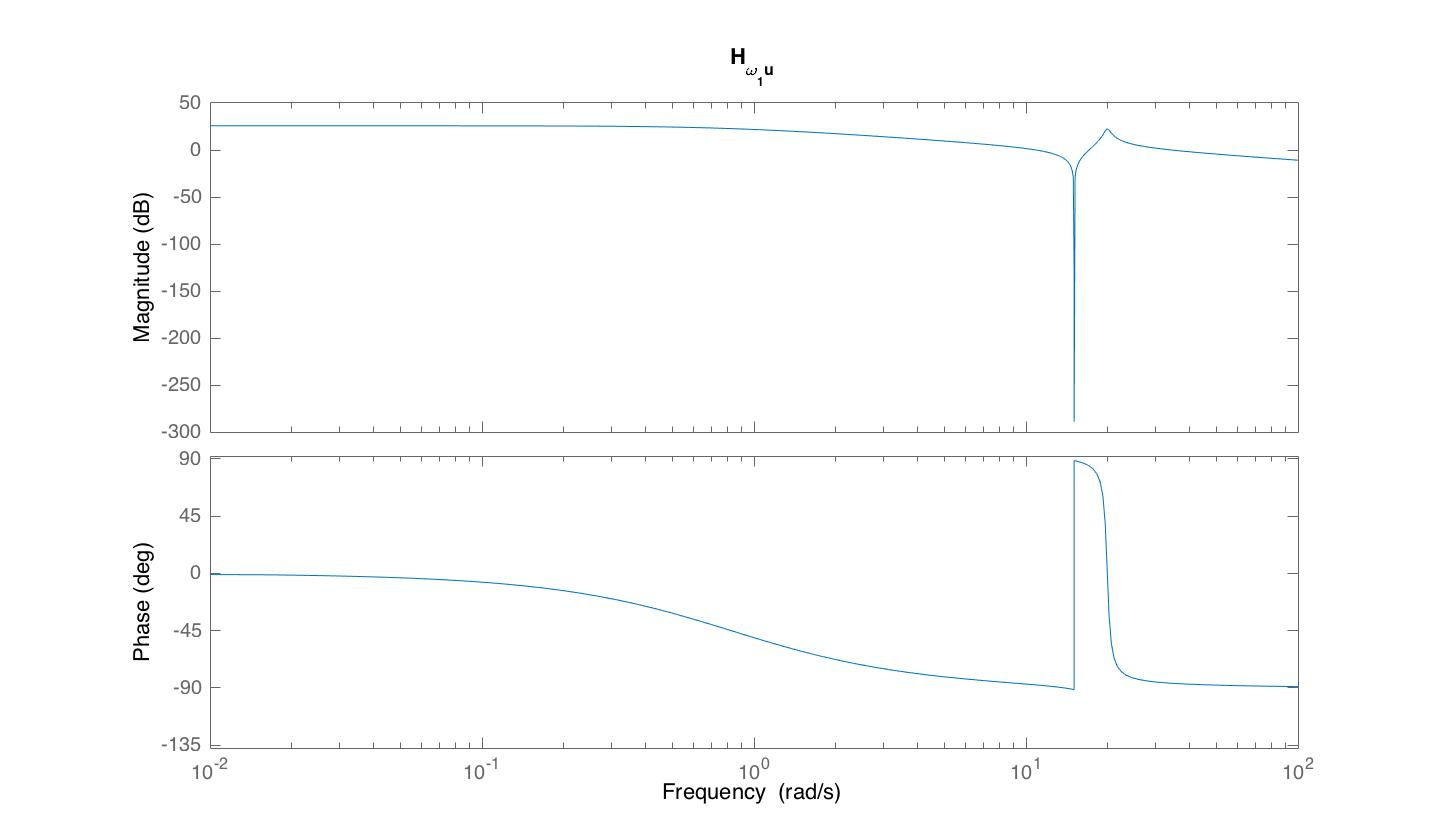
\includegraphics[trim={6cm 0 1cm 1cm},clip,origin=c,scale=0.26]{w1_bode}
            \caption{Frequency Response $H_{\omega_{1}u}$}
            \label{fig:disc_sys}
       \end{figure}
       
       \begin{figure}[H]
            \centering
            \begin{minipage}{.5\textwidth}
                \centering
              	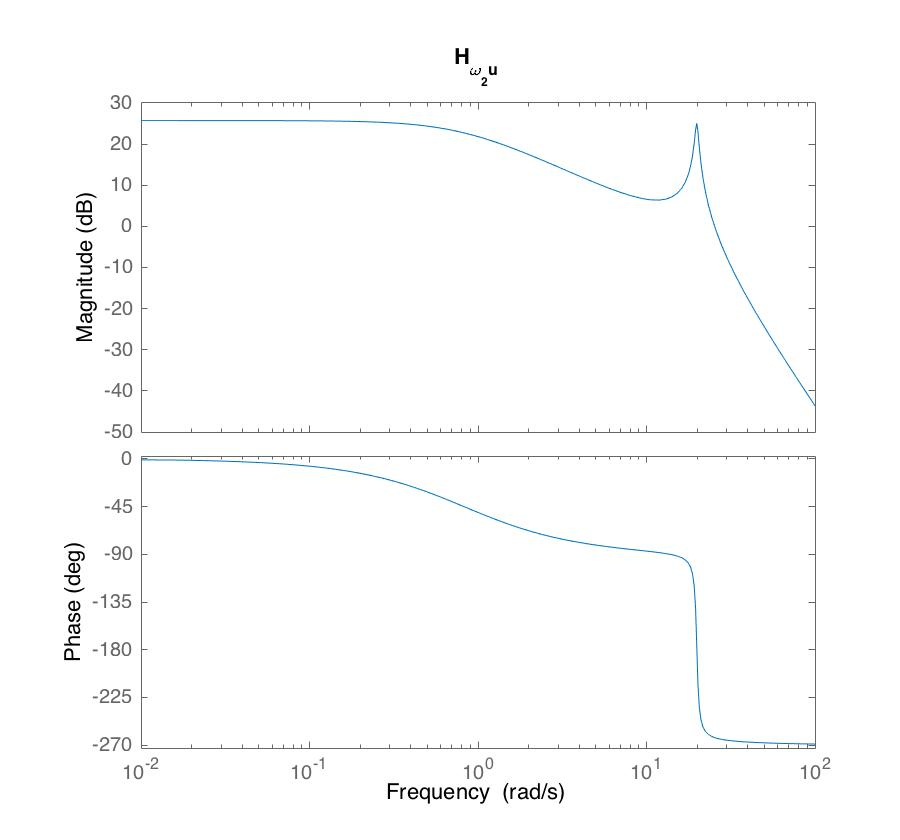
\includegraphics[trim={2cm 0 0 0},clip,origin=c,scale=0.25]{w2_bode}
            	\caption{Frequency Response $H_{\omega_{2}u}$}
           	\label{fig:disc_sys}
            \end{minipage}%
            \begin{minipage}{.5\textwidth}
                \centering
                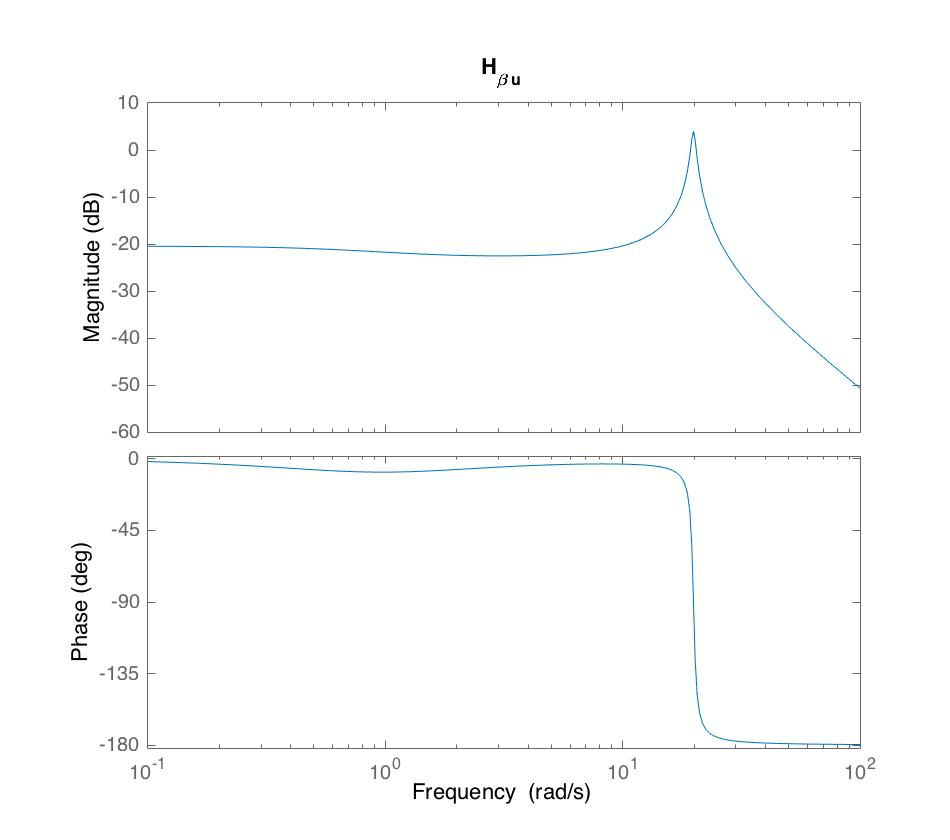
\includegraphics[trim={2cm 0 0 0},clip,origin=c,scale=0.25]{B_bode}
            \caption{Frequency Response $H_{\beta u}$}
            \label{fig:disc_sys}
            \end{minipage}%
       \end{figure}


\section{Least Squares Solutions}
	Another useful method for analyzing the TDS with two discs attached is to look at the frequency response of the system. After conducting the above conceptual analysis we obtained a good idea of how the system should respond to a sinusoidal input at different frequencies. To verify our assumptions we modified the Labview model to include a sinusoidal input and a proportional controller. For these experiments the $K_p$ value of the controller was kept small ($K_p = 1$ in our case). We then collected data for five different frequencies: 1Hz to 5Hz. The collected data provided the commanded voltage, the position of the bottom and middle discs, and a time vector. With this information we used the following equations to describe the system parameters.
	\subsection{Equations} \label{sec:eq}
		\begin{align}
			u(t) &= u_0 + u_{1a}cos(\omega_0t) + u_{1b}sin(\omega_0t) \\[1em]
			\Theta_1(t) &= \Theta_{10} + \omega_{10}t + \omega_{11a}\frac{sin(\omega_0t)}{\omega_0} - \omega_{11b}\frac{cos(\omega_0t)}{\omega_0} \\[1em]
			\Theta_2(t) &= \Theta_{20} + \omega_{20}t + \omega_{21a}\frac{sin(\omega_0t)}{\omega_0} - \omega_{21b}\frac{cos(\omega_0t)}{\omega_0} \\[1em]
			\omega_1(t) &= \omega_{10} + \omega_{11a}cos(w_0t) + \omega_{11b}sin(\omega_0t) \\[1em]
			\omega_2(t) &= \omega_{20} + \omega_{21a}cos(w_0t) + \omega_{21b}sin(\omega_0t)
		\end{align}
		Where $u(t)$ is the commanded motor voltage, $\Theta_1(t)$ is the bottom disc position, $\Theta_2(t)$ is the middle disc position, $\omega_1(t)$ is the bottom disc velocity, and $\omega_2(t)$ is the middle disc velocity.
	\subsection{Solutions Part I}
		With the above equations and the experimental data it is possible to set up and solve an overdetermined system using the Matlab command $x =A \setminus b$ where all unknowns are contained in the $x$ vector.
		\begin{equation}
			\begin{bmatrix}
				u_0 \\
				u_{1a} \\
				u_{1b}
			\end{bmatrix}
			=
			\begin{bmatrix}
				1 & cos(w_0t) & sin(w_0t) \\
			\end{bmatrix}
			\setminus
			\begin{bmatrix}
				u(t) \\
			\end{bmatrix}
		\end{equation} \\
		\begin{equation}
			\begin{bmatrix}
				\Theta_{10} \\
				\omega_{10} \\
				\omega_{11a} \\
				\omega_{11b}
			\end{bmatrix}
			=
			\begin{bmatrix}
				1 & t & \frac{sin(\omega_0t)}{\omega_0} & -\frac{cos(\omega_0t)}{\omega_0}
			\end{bmatrix}
			\setminus
			\begin{bmatrix}
				\Theta_1(t) \\
			\end{bmatrix}
		\end{equation} \\
		\begin{equation}
			\begin{bmatrix}
				\Theta_{20} \\
				\omega_{20} \\
				\omega_{21a} \\
				\omega_{21b}
			\end{bmatrix}
			=
			\begin{bmatrix}
				1 & t & \frac{sin(\omega_0t)}{\omega_0} & -\frac{cos(\omega_0t)}{\omega_0}
			\end{bmatrix}
			\setminus
			\begin{bmatrix}
				\Theta_2(t) \\
			\end{bmatrix}
		\end{equation}
		\begin{table}[H]
			\centering
			\begin{tabular}{|m{2cm}|m{2cm}|m{2cm}|m{2cm}|m{2cm}|m{2cm}|} 
			\hline
			Coefficient & 1Hz & 2Hz & 3Hz & 4Hz & 5Hz \\ 
			\hline
			$u_0$ & 0.1421 & 0.1388 & 0.1417 & 0.1444 & 0.1377 \\
			\hline
			$u_{1a}$ & 0.4018 & 0.6956 & -0.2100 & 0.5411 & 1.3734 \\
			\hline
			$u_{1b}$ & 0.0904 & 0.6801 & 0.5198 & -0.1373 & 0.5318 \\
			\hline
			$\Theta_{10}$ & -4.4558 & -4.5316 & -4.5296 & -4.5598 & -4.5868 \\
			\hline
			$\omega_{10}$ & 5.8560 & 5.8556 & 5.8557 & 5.8559 & 5.8598 \\
			\hline
			$\omega_{11a}$ & -0.2436 & -0.5921 & 0.4607 & 0.2722 & -0.9503 \\
			\hline
			$\omega_{11b}$ & 0.9809 & 0.5678 & 0.3671 & 1.5165 & 1.6875 \\
			\hline
			$\Theta_{20}$ & -4.4565 & -4.5295 & -4.5286 & -4.5609 & -4.5888 \\
			\hline
			$\omega_{20}$ & 5.8559 & 5.8552 & 5.8553 & 5.8559 & 5.8599 \\
			\hline
			$\omega_{21a}$ & -0.2876 & -1.4257 & -1.6382 & -0.2665 & 0.3443 \\
			\hline
			$\omega_{21b}$ & 1.1412 & 1.2872 & -0.9946 & -1.1456 & -0.6593 \\
			\hline
			\end{tabular}
			\caption{Coefficients} \label{table:coeff}
		\end{table}
	\subsection{Experimental Bode Plot} \label{sec:bode}
		The calculated values for the unknown coefficients shown in table \ref{table:coeff} can now be used to construct an experimental bode plot for the system. The transfer function of interest is shown in equation \ref{eq:tf} where $\hat{w_1}$ and $\hat{u}$ are the complex quantities at a specific frequency as defined below.
		\begin{align}
			H_{\omega_1u} &= \frac{\hat{\omega_1}(j\omega_0)}{\hat{u}(j\omega_0)} \label{eq:tf} \\[1em]
			\hat{u} &= u_{1a} - ju_{1b} \\[1em]
			\hat{\omega_1} &= \omega_{11a} - j\omega_{11b}
		\end{align}
		The experimental bode plot is shown below using Matlab's curve fitting toolbox for the five collected frequencies. This experimental does not exactly match the bode plots calculated in Matlab but the shape and key turning points are the same.
		\begin{figure}[H]
			\centering
			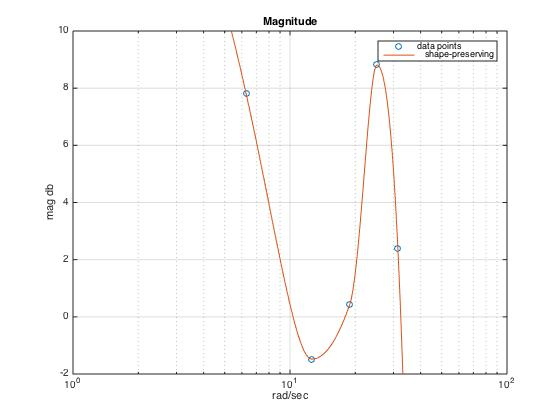
\includegraphics[scale=0.6]{experimentalBodeMag}
			\caption{Experimental Bode Plot Magnitude}
		\end{figure}
		\begin{figure}[H]
			\centering
			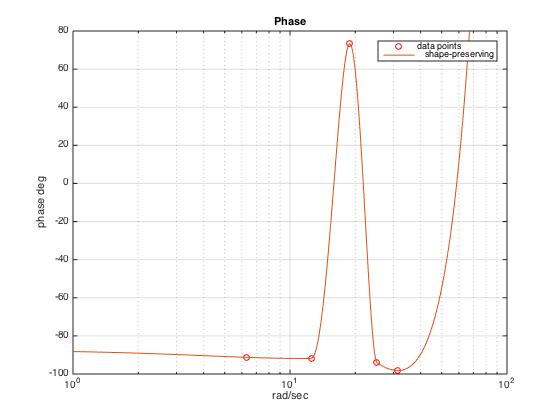
\includegraphics[scale=0.6]{experimentalBodePhase}
			\caption{Experimental Bode Plot Phase}
		\end{figure}
	\subsection{Solutions Part II}
		A final aspect pertaining to the frequency response was to use the least squares method to determine the unknown coefficients from the equations of motion. Adding the middle disc to the TDS system introduces new unknown parameters as shown in the below equations.
		\begin{align}
			J_1\dot{\omega_1} &+ c_1\omega_1 + k\beta - bu = 0 \\
			J_2\dot{\omega_2} &+ c_2\omega_2 -k\beta = 0 \\
			\dot{\beta} &= \omega_1 - \omega_2
		\end{align}
		The least squares equation $x =A \setminus b$ can again be used to solve for the unknowns in the $x$ vector. All other variables can be calculated from the equations in section \ref{sec:eq}.
		\begin{equation}
			\begin{bmatrix}
				c_1 \\
				k \\
				b \\
			\end{bmatrix}
			=
			\begin{bmatrix}
				\omega_1 & (\Theta_1 - \Theta_2) & -u \\
			\end{bmatrix}
			\setminus
			\begin{bmatrix}
				-J_1\dot{w_1}
			\end{bmatrix}
		\end{equation}\\
		\begin{equation}
			\begin{bmatrix}
				c_2 \\
				k
			\end{bmatrix}
			=
			\begin{bmatrix}
				w_2 & (\Theta_2 - \Theta_1) \\
			\end{bmatrix}
			\setminus
			\begin{bmatrix}
				-J_2\dot{w_2}
			\end{bmatrix}
		\end{equation}
		For the frequency $2\pi \mbox{ rad/sec}$ the calculated values are:
		\begin{align*}
			c_1 &= 0.00022632 \\
			c_2 &= 0.00010809 \\
			k &= 0.0117 \\
			b &= 0.0052 \\
		\end{align*}
		These values deviate from the calculated values using alternative methods but this could be due to noise in the experimental data or other unknowns.

	\section{Conclusion}
	It is useful to use multiple methods when experimentally determining system parameters and to compare the final results. In some cases taking and average of the results provides the best solution and in other cases it may become clear that one method is less robust and should be discarded. For the two disc TDS setup it is not clear at this point which method provides the more accurate results. It is necessary for us to explore this further in order to select the most accurate values. This lab introduced us to the least squares method for determining multiple unknowns. In addition, we determined essential parameters that will aid us in designing a controller for the 2 disc setup.

\end{document}